%FOR PDFLATEX USE ONLY
\documentclass[a4paper,12pt]{article}

\usepackage{amssymb,amsmath}

\usepackage[margin=2cm]{geometry}
\usepackage[unicode]{hyperref}
\usepackage[pdftex]{graphicx}
\usepackage{cmlgc}

\usepackage{array}

\usepackage{wrapfig}
\usepackage{array}
\usepackage{lipsum}
\usepackage{esvect}
\usepackage{hyperref}

\usepackage{subfig}
\usepackage{calc}
\usepackage{pgfplots,tikz,circuitikz}
\usepackage{pgfplotstable}
\usepackage{tkz-euclide}

\usepackage{centernot}
\usepackage{cancel}

\usepackage{mathtext}
\usepackage[T1,T2a]{fontenc}
\usepackage[utf8]{inputenc}
\usepackage[english, bulgarian, russian]{babel}
\usepackage{tikz}
\usepackage{pgfplots}
\usepackage[export]{adjustbox}
\usepackage[left=2cm,right=2cm,
    top=2cm,bottom=2cm,bindingoffset=0cm]{geometry}
\usepackage{indentfirst}
\usepackage{braket}

%\usepackage{centernot}
%\usepackage{cancel}

\begin{document}

\begin{center}
  \LARGE{Работа 1.2.1}\\[0.2cm]
  \LARGE{Определение скорости полета пули при помощи баллистического маятника}\\[0.2cm]
  \large{Панферов Андрей}\\[0.2cm]
\end{center}

\textbf{Цель работы:} определить скорость полета пули, применяя законы созранения и используя баллистические маятники.

\textbf{В работе используются:} духовое ружье на штативе, осветитель, оптическая система для измерения отклонений маятника, измерительная линейка, пули и весы для их взвенивания, а также баллистические маятники.

\section{Метод баллистического маятника, совершающего поступательное движение}

\begin{figure}[h]
\begin{center}$
\begin{array}{cc}
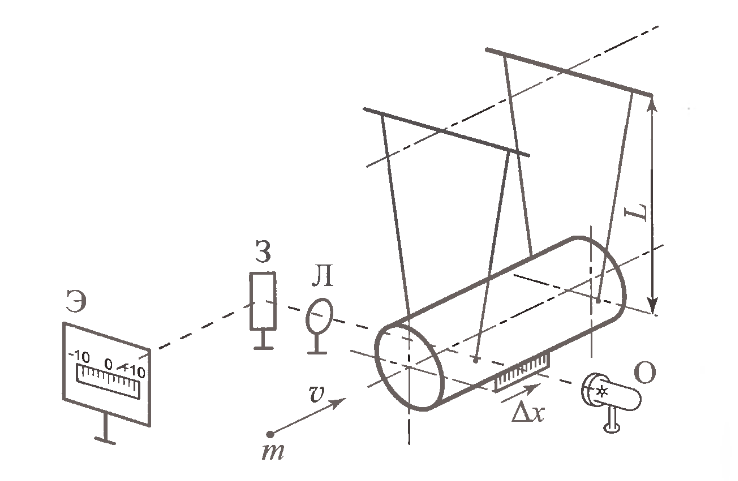
\includegraphics[width=0.45\textwidth]{prop-1.png}&
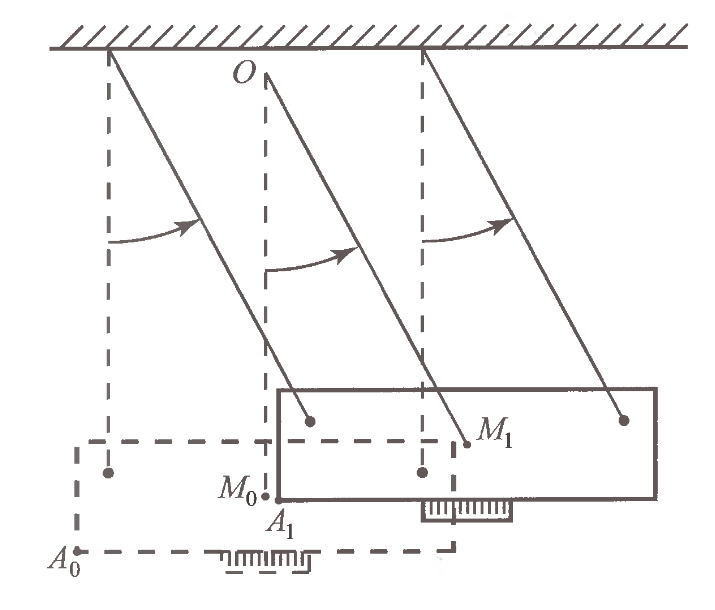
\includegraphics[width=0.45\textwidth]{prop-2.png}\\
\text{рис. 1, схема установки} & \text{рис. 2, поведение баллистического маятника}\\
&\text{при попадании в него пули.}
\end{array}$
\end{center}
\end{figure}
В этой части используется установка, изображенная на рис. 1. Если масса маятника равна $M$, то скорость системы маятник-пуля сразу после попадания маятника равна
\begin{equation}
v_0 = \frac{m}{M + m}v.
\end{equation}
У маятника угловая скорость $\omega = \sqrt{g/L}$. Если у него амплитуда $A$, то верно, что
\begin{equation}
A \omega = v_0.
\end{equation}
Из этого скорость выражается, как
\begin{equation}
v = \sqrt{\frac{g}{L}}\frac{M+m}{m}A.
\end{equation}
\newpage
\subsection{Результаты и обработка}

Массы пулек:
\begin{figure}[h]
\begin{center}$
\begin{array}{|c|c|c|c|c|c|c|c|c|}
\hline
N & 1 & 2 & 3 & 4 & 5 & 6 & 7 & 8  \\
\hline
m\text{, г} & 0.5061 & 0.5077 & 0.5091 & 0.4980 & 0.5134 & 0.5070 & 0.4995 & 0.5089  \\
\hline
\end{array}$
\end{center}
\caption*{$\Delta m = 0.001\text{г}$}
\end{figure}

$L = (2208\pm10)$ мм, $M=(2900\pm5)$ г.

Амплитуды и соответствующие скорости:

\begin{figure}[h]
\begin{center}$
\begin{array}{|c|c|}
\hline
A\text{, мм} & v\text{, м/c} \\
\hline
12.2\pm0.2 & 145\pm3 \\
\hline
12.2\pm0.2 & 146\pm3 \\
\hline
12.2\pm0.2 & 146\pm3 \\
\hline
12.2\pm0.2 & 145\pm3 \\
\hline
\end{array}$
\end{center}
\end{figure}

Усредняя, получаем $<v>=(146\pm3)\text{, м/c}$.

\section{Метод крутильного баллистического маятника}
В этом методе используется установка, изображенная на рис. 3.
\begin{figure}[h]
\begin{center}$
\begin{array}{c}
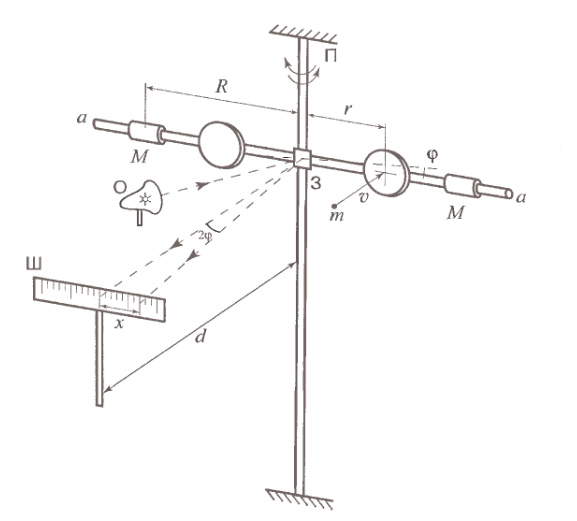
\includegraphics[width=0.73\textwidth]{rot.png}\\
\text{рис. 3, крутильный баллистический маятник.}
\end{array}$
\end{center}
\end{figure}
\newpage
Сразу после попадания пули в мишень, система пуля-мишень будет двигаться с угловой скоростью $\Omega$ такой, что
\begin{equation}
m v r = I \Omega,
\end{equation}
где $I$ -- момент инерции систему пуля-мишень.\\
Если $k$ -- модуль кручения проволоки, то из закона сохранения энергии следует, что
\begin{equation}
k \frac{\varphi^2}{2} = I \frac{\Omega^2}{2},
\end{equation}
где $\varphi$ -- амплитуда колебаний маятника после выстрела.
Из уравнений (4) и (5) можно найти скорость $v$ по амплитуде $\varphi$.
\begin{equation}
v = \varphi \frac{\sqrt{kI}}{mr}.
\end{equation}

Есть два метода расчета $\varphi$ -- простой и сложный.
\begin{equation}
\varphi_s = \frac{|x_0 - x_1|}{d}, \varphi_h = |atan(\frac{x_0}{d}) - atan(\frac{x_1}{d})| / 2.
\end{equation}

Если система колебается с периодом $T$, то верно, что ее момент инерции равен:

\begin{equation}
I = \frac{k}{4\pi^2}T^2.
\end{equation}

Если грузов на маятнике нет, то момент инерции системы обозначим за $I_0$. Если есть, то он равен

\begin{equation}
I = I_0 + 2 \Delta I + 2 M R^2,
\end{equation}

Где $M$ -- масса одного груза, a $\Delta I$ -- момент инерции груза относительно вертикальной оси, проходящей через его центр.

\subsection{Результаты и обработка}

Периоды колебаний

\begin{figure}[h]
\begin{center}$
\begin{tabular}{|c|c|c|c|c|c|}
\hline
С грузами, $10 \cdot T_1$, с&240&240&238&239&239\\
\hline
Без грузов, $10 \cdot T_2$, с&184&179&176&177&175\\
\hline
\end{tabular}$
\end{center}
\end{figure}

\begin{equation*}
\sqrt{\textit{kI}} = \frac{4 \pi M R^2 T_1}{T_1^2 - T_2^2} = (97 \pm 2)\cdot 10^{-2} \: kg \cdot m^2 / c сас
\end{equation*}


Из уравнений (10) можно найти $k = (0.0929\pm0.0003) \text{ кг$\cdot$м$^2/$c$^2$}$.

\begin{equation}
v = \varphi \frac{\sqrt{kI}}{mr} = \varphi \frac{kT}{2\pi mr}.
\end{equation}

\newpage
Амплитуды и скорости:

\begin{table}
\begin{center}
\begin{tabular}{|c|c|c|}
\hline
x, мм&$\varphi$, рад&v, м/с\\
\hline
135&0.182&143\\
\hline
140&0.189&152\\
\hline
131&0.177&143\\
\hline
132&0.178&141\\
\hline
\end{tabular}
\end{center}
\end{table}

Во 2 методе получается значение
$<v> = (145 \pm 6)\text{м/c}$.


В моей работе значения скоростей, полученные двумя разными методами, сходятся:
\begin{equation}
v_0 = (146 \pm 3)\text{м/c}, v_1 = (145 \pm 6)\text{м/c}.
\end{equation}

При этом я слышал, что у других людей на 2 установке получались значения скорости больше, чем на первой. Виной этому точно не неучет собственного момента инерции грузов в лабнике, поскольку во второй части у меня получилось, что он слишком мал. Также это не может происходить из-за приближения тангенса линейной функцией во 2 пункте, у меня отклонение финального ответа при линейном приближении получилось меньше процента от честного. Данный эффект может происходить из-за:
\begin{enumerate}
\item \text{Трения о воздух}
\item \text{Того, что по-настоящему этого эффекта нет -- все говорят, что он есть, но,}\\\text{честно промерив, его никто не получил, возможно, даже,}\\\text{некоторые студенты подогнали свои значения так, что этот эффект}\\\text{специально начал проявляться, что укрепило миф.}
\item \text{какой-то другой эффект, который не пришел мне в голову.}
\end{enumerate}
Рассмотрим трение о воздух. Диаметр пули равен $4.5\text{ мм}$, расстояние до цели порядка $80\text{ см}$ на различных установках, скорость пули порядка $140\text{ м$/$с}$. Посмотрим, насколько пуля замедлится.\\
Если брать квадратичную зависимость ($F=C_f\displaystyle \frac{\rho v^2}{2}S$) силы трения от скорости, то на пулю действует сила в $153\text{ мН}$, если считать пулю цилиндром. При массе в $0.5\text{ г}$, пуля успеет замедлиться на $1.7\text{ м/c}$ за это время. Поскольку порядок вариации расстояния от конца ствола до мишени -- $10\text{ см}$, что в 8 раз меньнше, получим вариацию в $0.2\text{ м/c}$ по скорости, что много меньше погрешности. Это не трение.
\section{Вывод}
Я получил значение скорости пули двумя методами -- методом баллистического маятника и методом крутильного маятника. Значения скорости совпали с точностью до погрешности. Физического объяснения того, что у других студентов получаются разные значения я не нашел, хотя рассмотрел три варианта: неучет момента инерции грузов, неучет нелинейности тангенса при расчете амплитуды отклонения и неучет силы трения о воздух.

\end{document}








\lipsum[1-4]
\begin{wrapfigure}{R}{5cm}
\centering
\includegraphics[width=0.20\textwidth]{rd.png}
\caption{1}
\end{wrapfigure}
\lipsum[1-6]


\begin{figure}[h]
\begin{center}$
\begin{array}{cccc}
\includegraphics[width=0.20\textwidth]{rd.png}&
\includegraphics[width=0.20\textwidth]{rd.png}&
\includegraphics[width=0.20\textwidth]{rd.png}&
\includegraphics[width=0.20\textwidth]{rd.png}\\
(1) & (2) & (3) & (4)
\end{array}$
\end{center}
\end{figure}
